\documentclass[12pt,a4paper]{article}

\usepackage[a4paper,text={16.5cm,25.2cm},centering]{geometry}
\usepackage{lmodern}
\usepackage{amssymb,amsmath}
\usepackage{bm}
\usepackage{graphicx}
\usepackage{microtype}
\usepackage{hyperref}
\setlength{\parindent}{0pt}
\setlength{\parskip}{1.2ex}

\usepackage[makeroom]{cancel}

\usepackage{import}
\usepackage{pdfpages}
\usepackage{transparent}
\usepackage{xcolor}

\newcommand{\incfig}[2][1]{%
    \def\svgwidth{#1\columnwidth}
    \import{./figures/}{#2.pdf_tex}
}

\pdfsuppresswarningpagegroup=1

\hypersetup
       {   pdfauthor = { Kevin Corcoran },
           pdftitle={ HW \#3 Report },
           colorlinks=TRUE,
           linkcolor=black,
           citecolor=blue,
           urlcolor=blue
       }

\title{ HW \#3 Report}

\author{ Kevin Corcoran }


\usepackage{upquote}
\usepackage{listings}
\usepackage{xcolor}
\lstset{
    basicstyle=\ttfamily\footnotesize,
    upquote=true,
    breaklines=true,
    breakindent=0pt,
    keepspaces=true,
    showspaces=false,
    columns=fullflexible,
    showtabs=false,
    showstringspaces=false,
    escapeinside={(*@}{@*)},
    extendedchars=true,
}
\newcommand{\HLJLt}[1]{#1}
\newcommand{\HLJLw}[1]{#1}
\newcommand{\HLJLe}[1]{#1}
\newcommand{\HLJLeB}[1]{#1}
\newcommand{\HLJLo}[1]{#1}
\newcommand{\HLJLk}[1]{\textcolor[RGB]{148,91,176}{\textbf{#1}}}
\newcommand{\HLJLkc}[1]{\textcolor[RGB]{59,151,46}{\textit{#1}}}
\newcommand{\HLJLkd}[1]{\textcolor[RGB]{214,102,97}{\textit{#1}}}
\newcommand{\HLJLkn}[1]{\textcolor[RGB]{148,91,176}{\textbf{#1}}}
\newcommand{\HLJLkp}[1]{\textcolor[RGB]{148,91,176}{\textbf{#1}}}
\newcommand{\HLJLkr}[1]{\textcolor[RGB]{148,91,176}{\textbf{#1}}}
\newcommand{\HLJLkt}[1]{\textcolor[RGB]{148,91,176}{\textbf{#1}}}
\newcommand{\HLJLn}[1]{#1}
\newcommand{\HLJLna}[1]{#1}
\newcommand{\HLJLnb}[1]{#1}
\newcommand{\HLJLnbp}[1]{#1}
\newcommand{\HLJLnc}[1]{#1}
\newcommand{\HLJLncB}[1]{#1}
\newcommand{\HLJLnd}[1]{\textcolor[RGB]{214,102,97}{#1}}
\newcommand{\HLJLne}[1]{#1}
\newcommand{\HLJLneB}[1]{#1}
\newcommand{\HLJLnf}[1]{\textcolor[RGB]{66,102,213}{#1}}
\newcommand{\HLJLnfm}[1]{\textcolor[RGB]{66,102,213}{#1}}
\newcommand{\HLJLnp}[1]{#1}
\newcommand{\HLJLnl}[1]{#1}
\newcommand{\HLJLnn}[1]{#1}
\newcommand{\HLJLno}[1]{#1}
\newcommand{\HLJLnt}[1]{#1}
\newcommand{\HLJLnv}[1]{#1}
\newcommand{\HLJLnvc}[1]{#1}
\newcommand{\HLJLnvg}[1]{#1}
\newcommand{\HLJLnvi}[1]{#1}
\newcommand{\HLJLnvm}[1]{#1}
\newcommand{\HLJLl}[1]{#1}
\newcommand{\HLJLld}[1]{\textcolor[RGB]{148,91,176}{\textit{#1}}}
\newcommand{\HLJLs}[1]{\textcolor[RGB]{201,61,57}{#1}}
\newcommand{\HLJLsa}[1]{\textcolor[RGB]{201,61,57}{#1}}
\newcommand{\HLJLsb}[1]{\textcolor[RGB]{201,61,57}{#1}}
\newcommand{\HLJLsc}[1]{\textcolor[RGB]{201,61,57}{#1}}
\newcommand{\HLJLsd}[1]{\textcolor[RGB]{201,61,57}{#1}}
\newcommand{\HLJLsdB}[1]{\textcolor[RGB]{201,61,57}{#1}}
\newcommand{\HLJLsdC}[1]{\textcolor[RGB]{201,61,57}{#1}}
\newcommand{\HLJLse}[1]{\textcolor[RGB]{59,151,46}{#1}}
\newcommand{\HLJLsh}[1]{\textcolor[RGB]{201,61,57}{#1}}
\newcommand{\HLJLsi}[1]{#1}
\newcommand{\HLJLso}[1]{\textcolor[RGB]{201,61,57}{#1}}
\newcommand{\HLJLsr}[1]{\textcolor[RGB]{201,61,57}{#1}}
\newcommand{\HLJLss}[1]{\textcolor[RGB]{201,61,57}{#1}}
\newcommand{\HLJLssB}[1]{\textcolor[RGB]{201,61,57}{#1}}
\newcommand{\HLJLnB}[1]{\textcolor[RGB]{59,151,46}{#1}}
\newcommand{\HLJLnbB}[1]{\textcolor[RGB]{59,151,46}{#1}}
\newcommand{\HLJLnfB}[1]{\textcolor[RGB]{59,151,46}{#1}}
\newcommand{\HLJLnh}[1]{\textcolor[RGB]{59,151,46}{#1}}
\newcommand{\HLJLni}[1]{\textcolor[RGB]{59,151,46}{#1}}
\newcommand{\HLJLnil}[1]{\textcolor[RGB]{59,151,46}{#1}}
\newcommand{\HLJLnoB}[1]{\textcolor[RGB]{59,151,46}{#1}}
\newcommand{\HLJLoB}[1]{\textcolor[RGB]{102,102,102}{\textbf{#1}}}
\newcommand{\HLJLow}[1]{\textcolor[RGB]{102,102,102}{\textbf{#1}}}
\newcommand{\HLJLp}[1]{#1}
\newcommand{\HLJLc}[1]{\textcolor[RGB]{153,153,119}{\textit{#1}}}
\newcommand{\HLJLch}[1]{\textcolor[RGB]{153,153,119}{\textit{#1}}}
\newcommand{\HLJLcm}[1]{\textcolor[RGB]{153,153,119}{\textit{#1}}}
\newcommand{\HLJLcp}[1]{\textcolor[RGB]{153,153,119}{\textit{#1}}}
\newcommand{\HLJLcpB}[1]{\textcolor[RGB]{153,153,119}{\textit{#1}}}
\newcommand{\HLJLcs}[1]{\textcolor[RGB]{153,153,119}{\textit{#1}}}
\newcommand{\HLJLcsB}[1]{\textcolor[RGB]{153,153,119}{\textit{#1}}}
\newcommand{\HLJLg}[1]{#1}
\newcommand{\HLJLgd}[1]{#1}
\newcommand{\HLJLge}[1]{#1}
\newcommand{\HLJLgeB}[1]{#1}
\newcommand{\HLJLgh}[1]{#1}
\newcommand{\HLJLgi}[1]{#1}
\newcommand{\HLJLgo}[1]{#1}
\newcommand{\HLJLgp}[1]{#1}
\newcommand{\HLJLgs}[1]{#1}
\newcommand{\HLJLgsB}[1]{#1}
\newcommand{\HLJLgt}[1]{#1}


\begin{document}

\maketitle

\section{Problem 1}%
\label{sec:problem_1}

\subsection{Part 1}%
\label{sub:part_1}

\par \textbf{Derive the stability function $\Phi (z)$ for the following} 


\begin{itemize}
  \item Predictor-corrector (Heun's)
    \[
      u_{n+1} = u_n + \frac{h}{2} \left(f(u_n,t_n) + f(u_n+hf(u_n,t_n),t_n)\right)
    .\] 

    \par For the model problem, $u'(t) = \gamma u(t)$, $f(u_n,t_n) = \gamma
    u_n$, and $f(u_n + h\gamma u_n)=\gamma(u_n+h\gamma u_n)$. So we have

    \begin{align*}
      u_{n+1} &= u_n + \frac{h}{2} \left(\gamma u_n + \gamma (u_n + h\gamma
      u_n) \right) \\
              &= \left(1 + h\gamma + \frac{(h\gamma)^2}{2}\right) u_n
    \end{align*}

    \par Define $z = h\gamma$, then the stability function $\Phi (z)$ is
    \[
      \boxed{\Phi (z) = 1 + z + \frac{z^2}{2}}
    .\] 

  \item $4$-th order Runge-Kutta

    \par For any Runga-Kutta method. Where $\vec{e}$ is a vector of all
    ones, we can write the general method in vector notation

    \begin{align*}
      \vec{k} &= f(u_n \vec{e} + hA\vec{k}) \\
      u_{n+1} &= u_{n} + h\vec{b}^T\vec{k} \\
    \end{align*}

    \par Then for the model problem, we have
    
    \begin{align*}
      \vec{k} &= \gamma u_{n}\vec{e}+ \gamma hA\vec{k} \\
      (I-zA)\vec{k} & = \gamma (I-zA)^{-1}u_{n}\vec{e} \\
      \implies \vec{k} &= \gamma (I-zA)^{-1} u_{n} \vec{e}
    \end{align*}

    \par and then,

    \begin{align*}
      u_{n+1} &= u_{n} + h\vec{b}^T\vec{k} \\
             &= u_{n} + z \vec{b}^{T} (I-zA)^{-1} u_{n} \vec{e} \\
             &= \left(1 +z \vec{b}^{T} (I-zA)^{-1}  \vec{e} \right) u_{n}
    \end{align*}

    \par So the stability function $\Phi (z)$ for any RK method is
    \[
    \boxed{\Phi (z) = 1 +z \vec{b}^{T} (I-zA)^{-1}  \vec{e}}
    .\] 

\end{itemize}

\subsection{Part 2}%
\label{sub:part_2}

\par \textbf{Study the zero-stability for each of the two LMMs below}

\begin{itemize}
  \item \[
      u_{n+2}-2u_{n+1} + u_{n} = hf(u_{n+1},t_{n+1}) - f(u_{n},t_{n})
  .\] 

  \par This has the following characteristic polynomial ($=0$)

  \begin{align*}
    \rho (\omega) &= \omega^{2} -2 \omega + 1 = 0 \\
                  &= ( \omega - 1)^{2} = 0
  \end{align*}

  With root $ \omega = 1$ of multiplicity $2$. Since this is not a simple root,
  this method is \textbf{not} zero stable.

\item \[
    u_{n+2} - u_{n} = h \left( \frac{1}{3} f(u_{n+2}, t_{n+2}) + \frac{4}{3}
    f(u_{n+1},t_{n+1}) + \frac{1}{3}f(u_n,t_n)\right)
.\] 

\par This method has characteristic polynomial 

\[
  \rho ( \omega) = \omega^{2} -1
.\] 

with roots 
\[
\omega = \pm 1
.\] 

Since $|w_i|\leq 1$, this method satisfies the root condition, and \textbf{is} therefore
zero stable.

\end{itemize}

\section{Problem 2}%
\label{sec:problem_2}

\subsection{Part 1}%
\label{sub:part_1}

\textbf{Show that 2s-DIRK is second order for $ \alpha = 1- \frac{1}{ \sqrt{2}}$} 

\par First order consistency condition 
\begin{align*}
  \sum^{p=2}_{i=1} b_i = 1 \\
  \implies (1 - \alpha) + \alpha = 1
\end{align*}

Which is satisfied regardless of the value of $ \alpha$.
\vspace{15px}
\par Second order consistency condition
\begin{align*}
  \sum^{p=2}_{i=1} b_i c_i &= \frac{1}{2} \\
  &= \underbrace{(1- \alpha)}_{b_1} \underbrace{\alpha}_{c_1}
  + \underbrace{\alpha}_{b_2} \underbrace{(1)}_{c_2} \\
  &= \frac{1}{\sqrt{2}} \left(1 - \frac{1}{\sqrt{2}}\right)
  + 1 - \frac{1}{\sqrt{2}} \\
  &= \frac{1}{2}
\end{align*}

So for $ \alpha = 1 - \frac{1}{\sqrt{2}}$, 2s-DIRK is at least second order.

\subsection{Part 2}%
\label{sub:part_2}

\par \textbf{For the model problem, $u' = \gamma u$, derive the expressions for
$k_1$, $k_2$, and the stability funciton $\Phi(z)$} 

\begin{align*}
  k_1 &= f(u_n + \alpha h k_1, t_n + \alpha h ) \\
      &= \gamma u_n + \alpha \gamma h k_1 \\
  \implies &\boxed{k_1 = \frac{ \gamma}{1- \alpha z }u_n}
\end{align*}

\begin{align*}
  k_2 &= f(u_n + h \left((1- \alpha) k_1 + a k_2\right), t_n + h) \\
      &= \gamma u_n + z \left((1- \alpha)\underbrace{\frac{ \gamma}{1- \alpha
      z }u_n}_{k_1} + \alpha k_2\right) \\
  \implies &\boxed{k_2 = \frac{(1- \alpha z) \gamma + \gamma z (1- \alpha)}{(1-
  \alpha z)^{2}} u_n}
\end{align*}

\par Then when $h$ is distributed in $u_{n+1} = u_{n} + \underbrace{h} ((1-
  \alpha)k_1 + \alpha k_2)$, we get $k_1$, and $k_2$ as desired.

  The stability function $\Phi$ follows from these results. Plugging in $k_1$
  and $k_2$
  
  \[
    u_{n+1} = \left(1 + (1- \alpha) \frac{z}{1- \alpha z } + \alpha \left(
    \frac{ (1- \alpha z)z + z^{2}(1- \alpha) }{(1- \alpha z)^{2}}
\right)\right) u_n
  .\] 

  So 
  \[
  \Phi(z) = 1 + (1- \alpha) \frac{z}{1- \alpha z } + \alpha \left(
    \frac{ (1- \alpha z)z + z^{2}(1- \alpha) }{(1- \alpha z)^{2}}
\right)
  .\] 

  \par Finding the common denominator and simplifying, we get the result as desired

  \[
    \boxed{\Phi(z) = \frac{ 1 + (1-2 \alpha)z }{(1- \alpha z)^{2}}}
  .\] 
\subsection{Part 3}%
\label{sub:part_3}

\par \textbf{Suppose 2s-DIRK is A-stable for $ \alpha
= 1 - \frac{1}{\sqrt{2}}$. Show that it satisfies the second condition of
L-stability} 

We want to show 
\[
  \lim_{z \to \infty} \Phi (z) = 0
.\] 

Make the change of variable $w = \frac{1}{z}$, then we can equivalently take
the limit as $w \to 0$

 \begin{align*}
   \lim_{w \to 0} \Phi(\frac{1}{w}) &= \lim_{w \to 0} \frac{ 1 + (1-2 \alpha) \frac{1}{w}
   }{(1 - \alpha \frac{1}{w})^{2}} \\
   &= \lim_{w \to 0} \frac{ w + (1-2 \alpha) }{w \frac{1}{w^{2}}(w- \alpha)^{2}} \\
   &= \lim_{w \to 0} \frac{ w^{2} + (1- 2 \alpha) w }{(w- \alpha)^{2}} \\
   &= 0
\end{align*}

So this method is L-stable.

\section{Problem 3}%
\label{sec:problem_3}

\par Consider the implicit 2-step method
\begin{align*}
  u_{n+2} - u_{n} &= h \left(\frac{1}{3}f(u_{n+2},t_{n+2})
  + \frac{4}{3}f(u_{n+1},t_{n+1}) + \frac{1}{3}f(u_{n},t_{n})\right) \\
\end{align*}

\subsection{Part 1}%
\label{sub:part_1}

\par \textbf{Show $e_n(h) = O(h^5)$}  

\par For the model problem 
\[
   \begin{cases}
     u'(t) = u(t) \\
     u(0) = 1
   \end{cases} \implies u(t) = e^{ t}
.\] 

\par the local truncation error 
\begin{align*}
  e_{n} &= \sum^{r}_{j=0} \alpha_{j}e^{ (t_{n}+jh)} - 
  h \sum^{r}_{j=1} \beta_{j}e^{ (t_{n}+jh)} \\
        &= e^{ t_{n}} \left( \sum \alpha_j e^{ jh} - \log(e^{jh})
        \sum \beta_j e^{ jh}\right)
\end{align*}

\par define $ z = e^{ h}$, then the order of the local truncation error
can be written in terms of $ z$
\[
  e_{n} = O(h^{p+1}) = O(\log( z)^{p+1}) \underbrace{=}_{\text{by Taylor
  expansion}} O( | z-1|^{p+1})
 .\] 


\par and more compactly, in terms of characteristic polynomials
 \begin{align}
   e_{n} &= \sum \alpha_j z^{j} - \log( z) \sum \beta_j z^{j} \\
         &= \rho( z) - \log( z) \sigma( z)
 \end{align}

 So now for this problem, we need to check the order of equation $(2)$. The
 characteristic polynomials are

 \begin{align*}
   \rho(z) = z^{2}-1 \\
   \sigma(z) = \frac{1}{3}z^{2} + \frac{4}{3}z + \frac{1}{3}
 \end{align*}

 let $ \zeta=z-1$, then
 
 \begin{align*}
   e_n &=\rho( \zeta + 1) - \log( \zeta + 1) \sigma( \zeta + 1) \\
        &= ( \zeta + 1)^{2} -1 -\log( \zeta + 1) \left( \frac{1}{3} ( \zeta
       +1)^{2} + \frac{4}{3}( \zeta + 1) + \frac{1}{3} \right)
 \end{align*}

 Taylor expanding $\log( \zeta+1)$

 \begin{align*}
   e_n &= \zeta^2 + 2 \zeta - \left( \zeta - \frac{\zeta^{2}}{2}
   + \frac{\zeta^{3}}{3} - \frac{\zeta^{4}}{4} + \frac{\zeta^{5}}{5} + O(
 \zeta^{6}) \left( \frac{1}{3} \zeta^{2} + 2 \zeta + 2\right)\right) \\
       &=\zeta^2 + 2 \zeta - \left(2 \zeta + \zeta^{2}(-1+2)
         + \zeta^{3}\cancel{(
         \frac{2}{3} -1 + \frac{1}{3})} + \zeta^{4}\cancel{(- \frac{1}{2} + \frac{2}{3}
       - \frac{1}{6})} + \zeta^{5} (\frac{2}{5}- \frac{1}{2} + \frac{1}{9}) + O(
   \zeta^{6})\right) \\
       &= \frac{1}{90} \zeta^{5} + O( \zeta^{6}) \\
       &= \frac{1}{90} (z-1)^{5} + O( (z-1)^{6}) \\
       &= O(h^{5})
 \end{align*}

 This shows that this implicit 2-step method is of order $5$.

 \subsection{Part 2}%
 \label{sub:part_2}

 \textbf{Find roots of the following for $z = - \epsilon$, $\epsilon > 0$} 
 \[
   \pi( \xi, z) = (\xi^{2} -1) - z\left(\frac{1}{3} \xi^{2}+ \frac{4}{3} \xi
   + \frac{1}{3}\right)
 .\] 

 Plugging in $z = -\epsilon$ and simplifying

  \begin{align*}
    \xi^{2} -1 + \epsilon \left( \frac{1}{3} \xi^{2} + \frac{4}{3} \xi
    + \frac{1}{3}\right) &= 0 \\
    \xi^{2} \left(1 + \frac{\epsilon}{3}\right) + \xi \left( \frac{4}{3}
  \epsilon\right) + \frac{\epsilon}{3} - 1 &= 0
 \end{align*}
 
 Using the quadratic formula and simpifying

 \begin{align*}
   \xi &= \frac{ - \frac{4}{3} \epsilon \pm ( \sqrt{(\frac{4}{3}\epsilon)^{2}
   - 4  (\frac{\epsilon}{3} + 1)( \frac{\epsilon}{3} -1)}}{2 (1
 + \frac{\epsilon}{3})} \\
       &= -\frac{2}{3} \epsilon \left( \frac{1}{1+ \frac{\epsilon}{3}}\right)
       \pm \frac{ \sqrt{ \frac{12}{9}\epsilon^{2}+4} }{2 (1+
       \frac{\epsilon}{3})} \\
       &= -\frac{2}{3} \epsilon \left( \frac{1}{1+ \frac{\epsilon}{3}}\right)
       \pm \frac{ \sqrt{1 + \frac{\epsilon}{3}} }{1 + \frac{\epsilon}{3}} \\
       &= -\frac{2}{3} \epsilon \left( \frac{1}{1+ \frac{\epsilon}{3}}\right)
       \pm \frac{1}{\sqrt{1 + \frac{\epsilon}{3}}}
 \end{align*}

 Now taylor expanding,

 \begin{align*}
   \xi &= - \frac{2}{3}\epsilon \left( 1- \frac{\epsilon}{3} + O(
   \epsilon^{2})\right) \pm 1 - \frac{\epsilon}{6} + O(\epsilon^{2})
 \end{align*}

 Gives us the roots
  \[
    \xi_1 (\epsilon) = 1 - \frac{5}{6}\epsilon + O(\epsilon^{2}), \qquad \xi_2
    = - \left(1 + \frac{1}{3}\right) + O(\epsilon^{2})
  .\] 

  Since $|\xi_i|\nleq 1$, the root condition is not satisfied, and so
  $z=-\epsilon$ is \textbf{not} in the region of absolute stability.

\section{Including required packages}

\begin{lstlisting}
(*@\HLJLk{using}@*) (*@\HLJLn{Plots}@*)
(*@\HLJLk{using}@*) (*@\HLJLn{LaTeXStrings}@*)
(*@\HLJLnf{theme}@*)(*@\HLJLp{(}@*)(*@\HLJLsc{:mute}@*)(*@\HLJLp{)}@*)

(*@\HLJLk{using}@*) (*@\HLJLn{Pkg}@*)
(*@\HLJLn{Pkg}@*)(*@\HLJLoB{.}@*)(*@\HLJLnf{activate}@*)(*@\HLJLp{(}@*)(*@\HLJLs{"{}RAS"{}}@*)(*@\HLJLp{)}@*)
(*@\HLJLnf{include}@*)(*@\HLJLp{(}@*)(*@\HLJLs{"{}code/RAS.jl"{}}@*)(*@\HLJLp{)}@*) (*@\HLJLcs{{\#}}@*) (*@\HLJLcs{Makes}@*) (*@\HLJLcs{sure}@*) (*@\HLJLcs{the}@*) (*@\HLJLcs{module}@*) (*@\HLJLcs{is}@*) (*@\HLJLcs{run}@*) (*@\HLJLcs{before}@*) (*@\HLJLcs{using}@*) (*@\HLJLcs{it}@*)
(*@\HLJLk{using}@*) (*@\HLJLoB{.}@*)(*@\HLJLn{RAS}@*)(*@\HLJLoB{:}@*) (*@\HLJLn{RAS{\_}stabf}@*)(*@\HLJLp{,}@*) (*@\HLJLn{RASrk}@*)

(*@\HLJLn{Pkg}@*)(*@\HLJLoB{.}@*)(*@\HLJLnf{activate}@*)(*@\HLJLp{(}@*)(*@\HLJLs{"{}DiffyQ"{}}@*)(*@\HLJLp{)}@*)
(*@\HLJLnf{include}@*)(*@\HLJLp{(}@*)(*@\HLJLs{"{}code/DiffyQ.jl"{}}@*)(*@\HLJLp{)}@*) (*@\HLJLcs{{\#}}@*) (*@\HLJLcs{Makes}@*) (*@\HLJLcs{sure}@*) (*@\HLJLcs{the}@*) (*@\HLJLcs{module}@*) (*@\HLJLcs{is}@*) (*@\HLJLcs{run}@*) (*@\HLJLcs{before}@*) (*@\HLJLcs{using}@*) (*@\HLJLcs{it}@*)
(*@\HLJLk{using}@*) (*@\HLJLoB{.}@*)(*@\HLJLn{DiffyQ}@*)(*@\HLJLoB{:}@*) (*@\HLJLn{s2{\_}DIRK}@*)(*@\HLJLp{,}@*) (*@\HLJLn{BackwardEuler{\_}n}@*)
\end{lstlisting}


\section{Problem 4: Plot Region of Absolute Stability}
Note that "light" color is the region of stability


\begin{lstlisting}
(*@\HLJLcs{{\#}}@*) (*@\HLJLcs{stability}@*) (*@\HLJLcs{function}@*) (*@\HLJLcs{for}@*) (*@\HLJLcs{Heun{\textquotesingle}s}@*)
(*@\HLJLnf{\ensuremath{\Phi}}@*)(*@\HLJLp{(}@*)(*@\HLJLn{z}@*)(*@\HLJLp{)}@*) (*@\HLJLoB{=}@*) (*@\HLJLnfB{1.0}@*) (*@\HLJLoB{+}@*) (*@\HLJLn{z}@*) (*@\HLJLoB{+}@*) (*@\HLJLn{z}@*)(*@\HLJLoB{{\textasciicircum}}@*)(*@\HLJLni{2}@*)
(*@\HLJLn{xs}@*)(*@\HLJLp{,}@*) (*@\HLJLn{Z}@*) (*@\HLJLoB{=}@*) (*@\HLJLnf{RAS{\_}stabf}@*)(*@\HLJLp{(}@*)(*@\HLJLn{\ensuremath{\Phi}}@*)(*@\HLJLp{)}@*)

(*@\HLJLnf{contourf}@*)(*@\HLJLp{(}@*)(*@\HLJLn{xs}@*)(*@\HLJLp{,}@*) (*@\HLJLn{xs}@*)(*@\HLJLp{,}@*) (*@\HLJLn{Z}@*)(*@\HLJLp{,}@*) (*@\HLJLn{levels}@*) (*@\HLJLoB{=}@*) (*@\HLJLni{1}@*)(*@\HLJLp{)}@*)
\end{lstlisting}

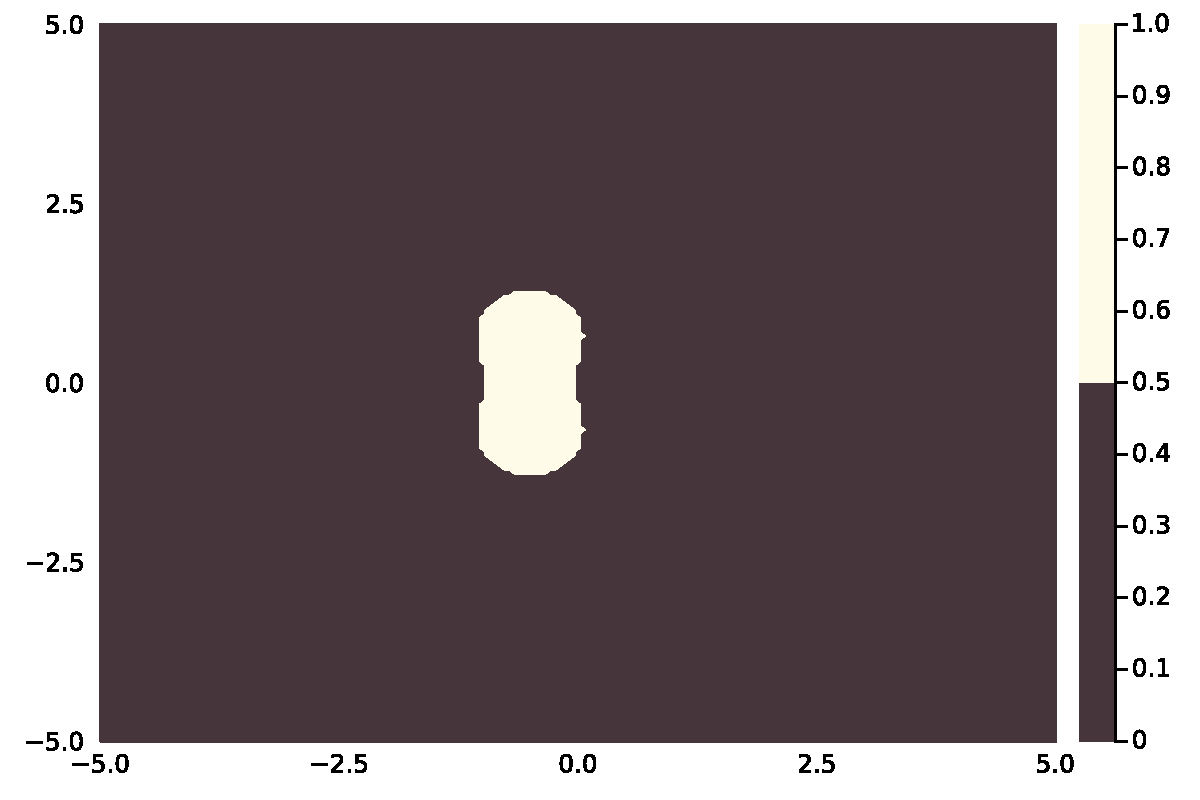
\includegraphics[width=\linewidth]{figures/ass_3_report_2_1.pdf}

\begin{lstlisting}
(*@\HLJLcs{{\#}}@*) (*@\HLJLcs{RK4}@*)
(*@\HLJLn{A}@*) (*@\HLJLoB{=}@*) (*@\HLJLp{[}@*)(*@\HLJLni{0}@*) (*@\HLJLni{0}@*) (*@\HLJLni{0}@*) (*@\HLJLni{0}@*)
    (*@\HLJLni{1}@*)(*@\HLJLoB{/}@*)(*@\HLJLni{2}@*) (*@\HLJLni{0}@*) (*@\HLJLni{0}@*) (*@\HLJLni{0}@*)
    (*@\HLJLni{0}@*) (*@\HLJLni{1}@*)(*@\HLJLoB{/}@*)(*@\HLJLni{2}@*) (*@\HLJLni{0}@*) (*@\HLJLni{0}@*)
    (*@\HLJLni{0}@*) (*@\HLJLni{0}@*) (*@\HLJLni{1}@*) (*@\HLJLni{0}@*)(*@\HLJLp{]}@*)
(*@\HLJLn{b}@*) (*@\HLJLoB{=}@*) (*@\HLJLp{[}@*)(*@\HLJLni{1}@*)(*@\HLJLoB{/}@*)(*@\HLJLni{6}@*)(*@\HLJLp{,}@*) (*@\HLJLni{1}@*)(*@\HLJLoB{/}@*)(*@\HLJLni{3}@*)(*@\HLJLp{,}@*) (*@\HLJLni{1}@*)(*@\HLJLoB{/}@*)(*@\HLJLni{3}@*)(*@\HLJLp{,}@*) (*@\HLJLni{1}@*)(*@\HLJLoB{/}@*)(*@\HLJLni{6}@*)(*@\HLJLp{]}@*)

(*@\HLJLn{xs}@*)(*@\HLJLp{,}@*) (*@\HLJLn{Z}@*) (*@\HLJLoB{=}@*) (*@\HLJLnf{RASrk}@*)(*@\HLJLp{(}@*)(*@\HLJLn{A}@*)(*@\HLJLp{,}@*)(*@\HLJLn{b}@*)(*@\HLJLp{)}@*)
(*@\HLJLcs{{\#}}@*) (*@\HLJLcs{plotly()}@*)
(*@\HLJLnf{contourf}@*)(*@\HLJLp{(}@*)(*@\HLJLn{xs}@*)(*@\HLJLp{,}@*)(*@\HLJLn{xs}@*)(*@\HLJLp{,}@*)(*@\HLJLn{Z}@*)(*@\HLJLp{,}@*) (*@\HLJLn{levels}@*) (*@\HLJLoB{=}@*) (*@\HLJLni{1}@*)(*@\HLJLp{)}@*)
\end{lstlisting}

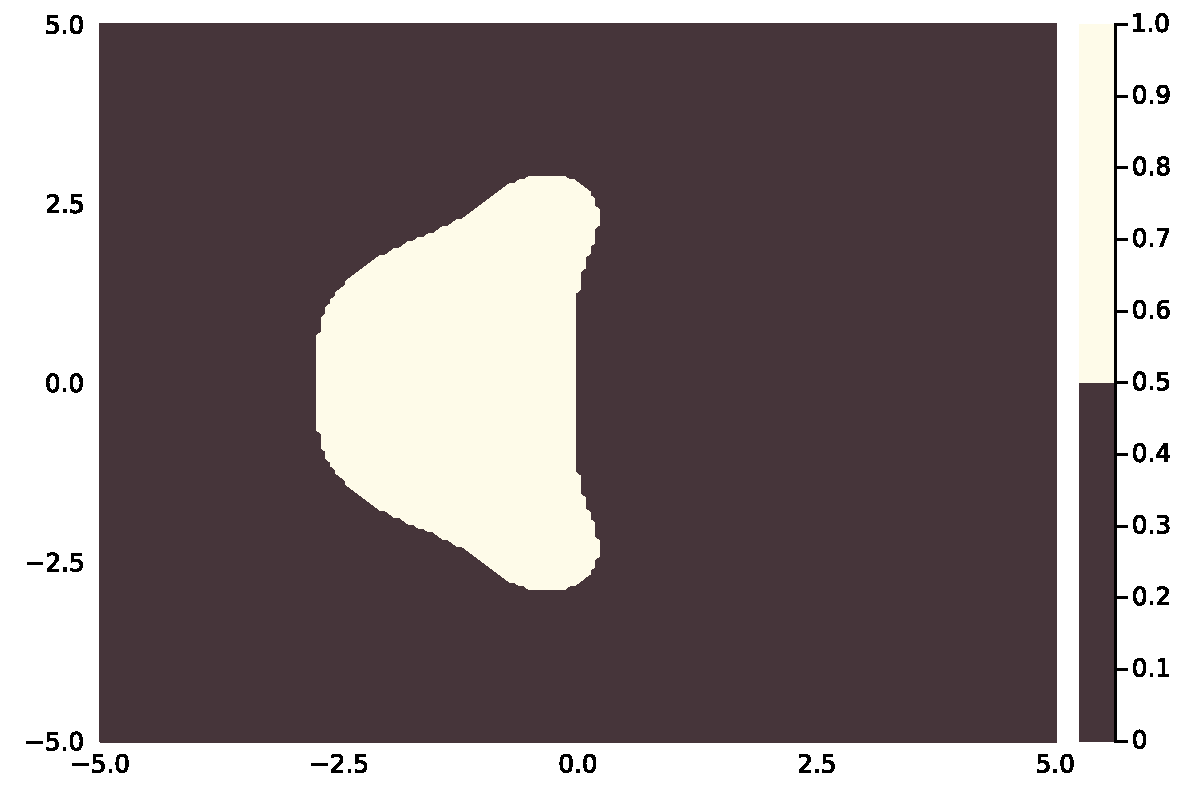
\includegraphics[width=\linewidth]{figures/ass_3_report_3_1.pdf}

\begin{lstlisting}
(*@\HLJLcs{{\#}}@*) (*@\HLJLcs{2s-DIRK}@*)
(*@\HLJLn{\ensuremath{\alpha}}@*) (*@\HLJLoB{=}@*) (*@\HLJLni{1}@*)(*@\HLJLoB{-}@*)(*@\HLJLni{1}@*)(*@\HLJLoB{/}@*)(*@\HLJLnf{sqrt}@*)(*@\HLJLp{(}@*)(*@\HLJLni{2}@*)(*@\HLJLp{)}@*)
(*@\HLJLn{A}@*) (*@\HLJLoB{=}@*) (*@\HLJLp{[}@*)(*@\HLJLn{\ensuremath{\alpha}}@*) (*@\HLJLni{0}@*)
    (*@\HLJLni{1}@*)(*@\HLJLoB{-}@*)(*@\HLJLn{\ensuremath{\alpha}}@*) (*@\HLJLn{\ensuremath{\alpha}}@*)(*@\HLJLp{]}@*)
(*@\HLJLn{b}@*) (*@\HLJLoB{=}@*) (*@\HLJLp{[}@*)(*@\HLJLni{1}@*)(*@\HLJLoB{-}@*)(*@\HLJLn{\ensuremath{\alpha}}@*)(*@\HLJLp{,}@*) (*@\HLJLn{\ensuremath{\alpha}}@*)(*@\HLJLp{]}@*)

(*@\HLJLn{xs}@*)(*@\HLJLp{,}@*) (*@\HLJLn{Z}@*) (*@\HLJLoB{=}@*) (*@\HLJLnf{RASrk}@*)(*@\HLJLp{(}@*)(*@\HLJLn{A}@*)(*@\HLJLp{,}@*)(*@\HLJLn{b}@*)(*@\HLJLp{)}@*)
(*@\HLJLnf{contourf}@*)(*@\HLJLp{(}@*)(*@\HLJLn{xs}@*)(*@\HLJLp{,}@*)(*@\HLJLn{xs}@*)(*@\HLJLp{,}@*)(*@\HLJLn{Z}@*)(*@\HLJLp{,}@*) (*@\HLJLn{levels}@*) (*@\HLJLoB{=}@*) (*@\HLJLni{1}@*)(*@\HLJLp{)}@*)
\end{lstlisting}

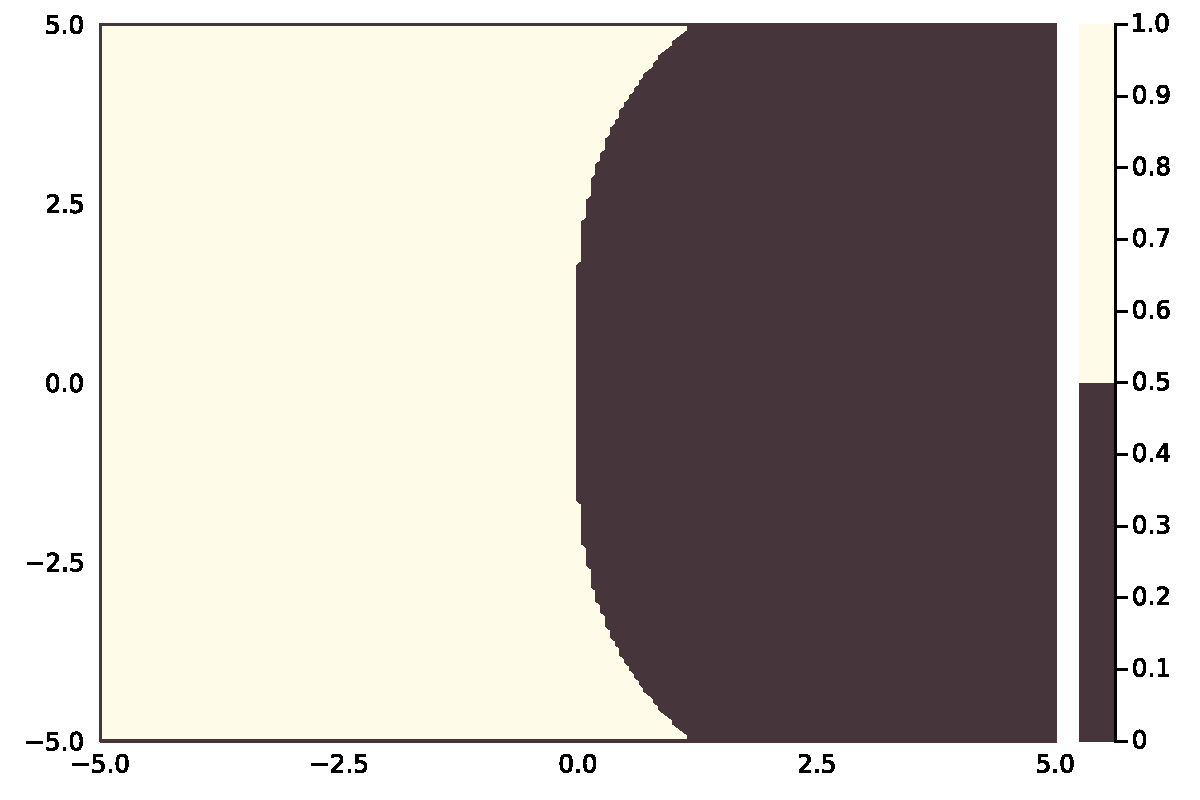
\includegraphics[width=\linewidth]{figures/ass_3_report_4_1.pdf}

\begin{lstlisting}
(*@\HLJLcs{{\#}}@*) (*@\HLJLcs{2s-DIRK}@*)
(*@\HLJLn{\ensuremath{\alpha}}@*) (*@\HLJLoB{=}@*) (*@\HLJLnfB{0.5}@*)
(*@\HLJLn{A}@*) (*@\HLJLoB{=}@*) (*@\HLJLp{[}@*)(*@\HLJLn{\ensuremath{\alpha}}@*) (*@\HLJLni{0}@*)
    (*@\HLJLni{1}@*)(*@\HLJLoB{-}@*)(*@\HLJLn{\ensuremath{\alpha}}@*) (*@\HLJLn{\ensuremath{\alpha}}@*)(*@\HLJLp{]}@*)
(*@\HLJLn{b}@*) (*@\HLJLoB{=}@*) (*@\HLJLp{[}@*)(*@\HLJLni{1}@*)(*@\HLJLoB{-}@*)(*@\HLJLn{\ensuremath{\alpha}}@*)(*@\HLJLp{,}@*) (*@\HLJLn{\ensuremath{\alpha}}@*)(*@\HLJLp{]}@*)

(*@\HLJLn{xs}@*)(*@\HLJLp{,}@*) (*@\HLJLn{Z}@*) (*@\HLJLoB{=}@*) (*@\HLJLnf{RASrk}@*)(*@\HLJLp{(}@*)(*@\HLJLn{A}@*)(*@\HLJLp{,}@*)(*@\HLJLn{b}@*)(*@\HLJLp{)}@*)
(*@\HLJLnf{contourf}@*)(*@\HLJLp{(}@*)(*@\HLJLn{xs}@*)(*@\HLJLp{,}@*)(*@\HLJLn{xs}@*)(*@\HLJLp{,}@*)(*@\HLJLn{Z}@*)(*@\HLJLp{,}@*) (*@\HLJLn{levels}@*) (*@\HLJLoB{=}@*) (*@\HLJLni{1}@*)(*@\HLJLp{)}@*)
\end{lstlisting}

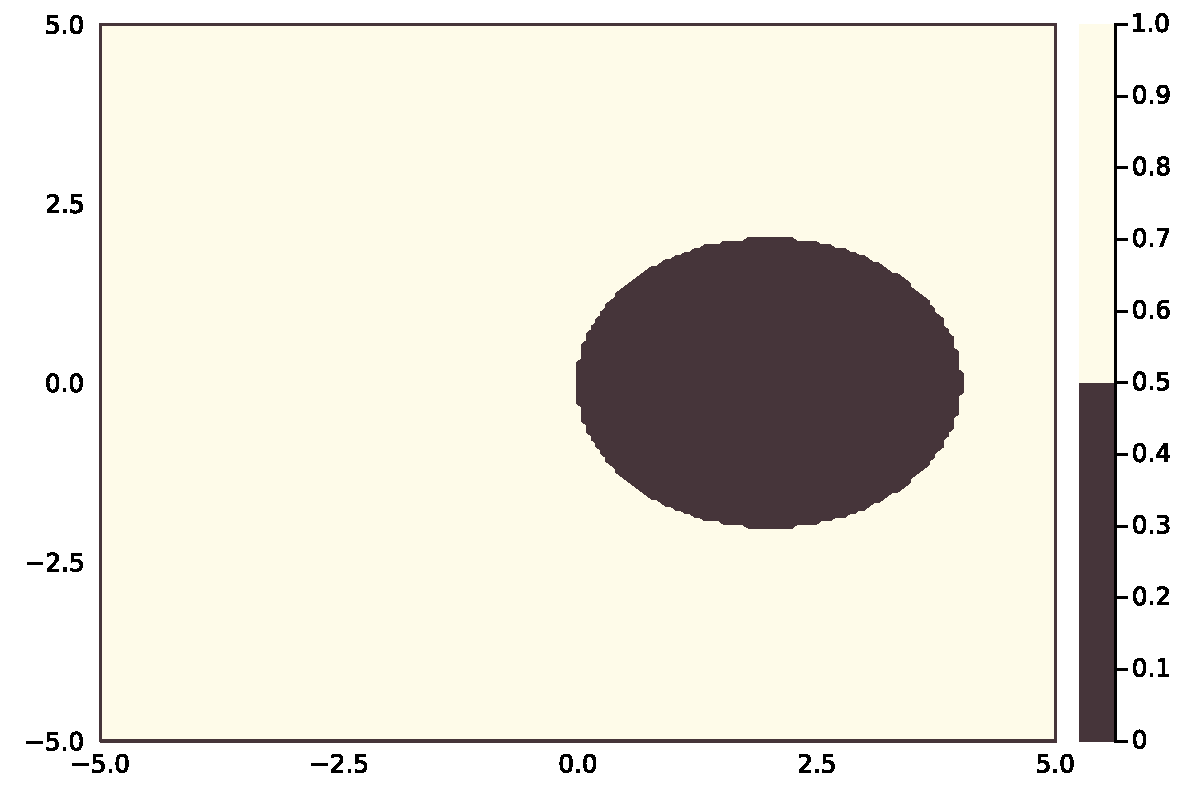
\includegraphics[width=\linewidth]{figures/ass_3_report_5_1.pdf}

\section{Problem 5}

\begin{lstlisting}
(*@\HLJLnf{f}@*)(*@\HLJLp{(}@*)(*@\HLJLn{u}@*)(*@\HLJLp{,}@*)(*@\HLJLn{t}@*)(*@\HLJLp{,}@*)(*@\HLJLn{\ensuremath{\mu}}@*)(*@\HLJLp{)}@*) (*@\HLJLoB{=}@*) (*@\HLJLoB{-}@*)(*@\HLJLp{(}@*)(*@\HLJLnfB{0.5}@*)(*@\HLJLoB{*}@*)(*@\HLJLnf{exp}@*)(*@\HLJLp{(}@*)(*@\HLJLni{20}@*)(*@\HLJLoB{*}@*)(*@\HLJLnf{cos}@*)(*@\HLJLp{(}@*)(*@\HLJLnfB{1.3}@*)(*@\HLJLoB{*}@*)(*@\HLJLn{t}@*)(*@\HLJLp{))}@*) (*@\HLJLoB{*}@*) (*@\HLJLnf{sinh}@*)(*@\HLJLp{(}@*)(*@\HLJLn{u}@*)(*@\HLJLoB{-}@*)(*@\HLJLnf{cos}@*)(*@\HLJLp{(}@*)(*@\HLJLn{t}@*)(*@\HLJLp{)));}@*)

(*@\HLJLn{\ensuremath{\alpha}}@*) (*@\HLJLoB{=}@*) (*@\HLJLni{1}@*) (*@\HLJLoB{-}@*) (*@\HLJLni{1}@*)(*@\HLJLoB{/}@*)(*@\HLJLnf{sqrt}@*)(*@\HLJLp{(}@*)(*@\HLJLni{2}@*)(*@\HLJLp{);}@*)
(*@\HLJLn{T}@*) (*@\HLJLoB{=}@*) (*@\HLJLnfB{30.0}@*)(*@\HLJLp{;}@*) (*@\HLJLn{h}@*) (*@\HLJLoB{=}@*) (*@\HLJLnfB{2.0}@*)(*@\HLJLoB{{\textasciicircum}}@*)(*@\HLJLp{(}@*)(*@\HLJLoB{-}@*)(*@\HLJLni{5}@*)(*@\HLJLp{);}@*) (*@\HLJLn{N}@*) (*@\HLJLoB{=}@*) (*@\HLJLnf{Int}@*)(*@\HLJLp{(}@*)(*@\HLJLn{T}@*)(*@\HLJLoB{/}@*)(*@\HLJLn{h}@*)(*@\HLJLp{);}@*)
(*@\HLJLn{u0}@*) (*@\HLJLoB{=}@*) (*@\HLJLnfB{0.0}@*)(*@\HLJLp{;}@*)

(*@\HLJLn{u}@*) (*@\HLJLoB{=}@*) (*@\HLJLnf{s2{\_}DIRK}@*)(*@\HLJLp{(}@*)(*@\HLJLn{f}@*)(*@\HLJLp{,}@*) (*@\HLJLn{N}@*)(*@\HLJLp{,}@*) (*@\HLJLn{T}@*)(*@\HLJLp{,}@*) (*@\HLJLn{u0}@*)(*@\HLJLp{,}@*) (*@\HLJLn{\ensuremath{\alpha}}@*)(*@\HLJLp{);}@*)
\end{lstlisting}


\subsection{Part 1}

\begin{lstlisting}
(*@\HLJLn{tList}@*) (*@\HLJLoB{=}@*) (*@\HLJLnf{collect}@*)(*@\HLJLp{(}@*)(*@\HLJLni{0}@*)(*@\HLJLoB{:}@*)(*@\HLJLn{N}@*)(*@\HLJLp{)}@*)(*@\HLJLoB{*}@*)(*@\HLJLp{(}@*)(*@\HLJLn{T}@*)(*@\HLJLoB{/}@*)(*@\HLJLn{N}@*)(*@\HLJLp{)}@*)
(*@\HLJLnf{plot}@*)(*@\HLJLp{(}@*)(*@\HLJLn{tList}@*)(*@\HLJLp{,}@*) (*@\HLJLn{u}@*)(*@\HLJLp{,}@*) (*@\HLJLn{label}@*) (*@\HLJLoB{=}@*) (*@\HLJLso{L"{}u(t)"{}}@*)(*@\HLJLp{,}@*) (*@\HLJLn{thickness{\_}scaling}@*) (*@\HLJLoB{=}@*)(*@\HLJLnfB{1.25}@*)(*@\HLJLp{)}@*)
(*@\HLJLnf{xlabel!}@*)(*@\HLJLp{(}@*)(*@\HLJLso{L"{}t"{}}@*)(*@\HLJLp{)}@*)
(*@\HLJLnf{ylabel!}@*)(*@\HLJLp{(}@*)(*@\HLJLso{L"{}u(t)"{}}@*)(*@\HLJLp{)}@*)
(*@\HLJLnf{title!}@*)(*@\HLJLp{(}@*)(*@\HLJLnf{latexstring}@*)(*@\HLJLp{(}@*)(*@\HLJLs{"{}2s-DIRK,h=2{\textasciicircum}{\{}-5{\}},T="{}}@*)(*@\HLJLp{,}@*)(*@\HLJLn{T}@*)(*@\HLJLp{))}@*)
(*@\HLJLnf{plot!}@*)(*@\HLJLp{(}@*)(*@\HLJLn{tList}@*)(*@\HLJLp{,}@*) (*@\HLJLn{cos}@*)(*@\HLJLoB{.}@*)(*@\HLJLp{(}@*)(*@\HLJLn{tList}@*)(*@\HLJLp{),}@*) (*@\HLJLn{label}@*) (*@\HLJLoB{=}@*) (*@\HLJLso{L"{}cos(t)"{}}@*)(*@\HLJLp{)}@*)
\end{lstlisting}

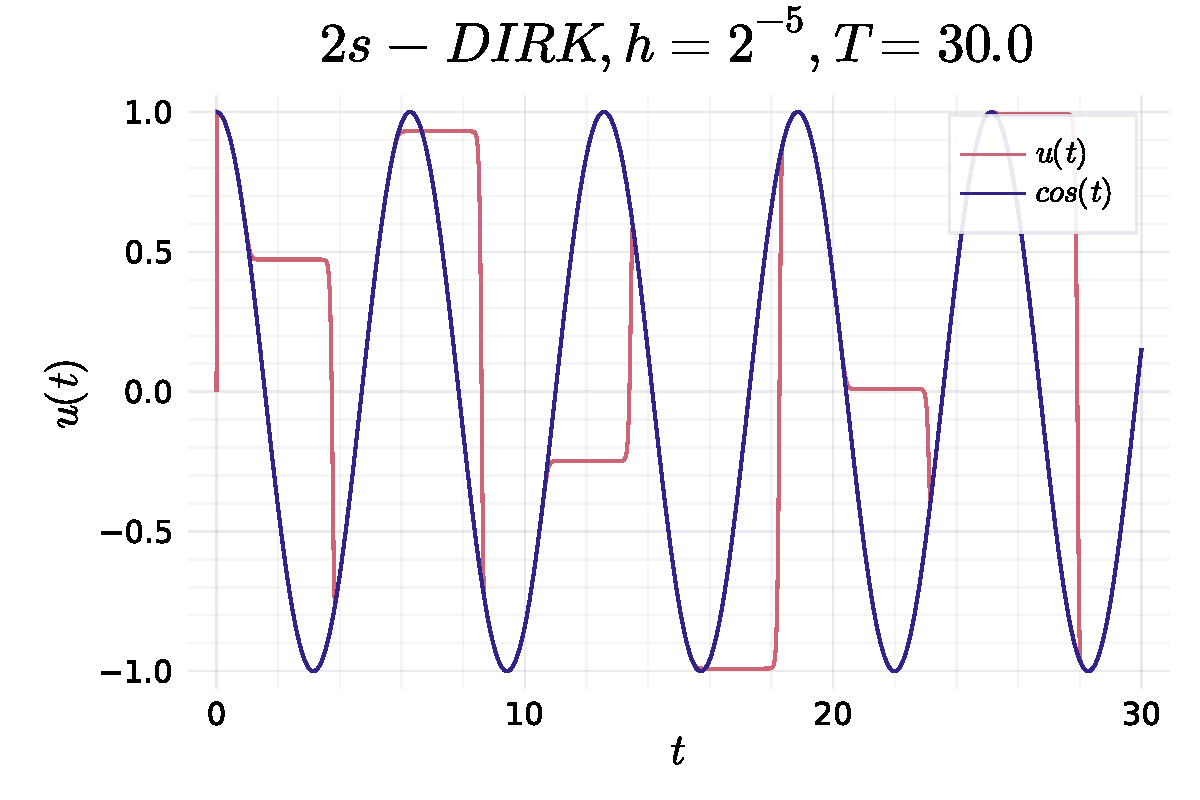
\includegraphics[width=\linewidth]{figures/ass_3_report_7_1.pdf}

\subsection{Part 2}

\begin{lstlisting}
(*@\HLJLnf{g}@*)(*@\HLJLp{(}@*)(*@\HLJLn{t}@*)(*@\HLJLp{)}@*) (*@\HLJLoB{=}@*) (*@\HLJLnfB{0.5}@*)(*@\HLJLoB{*}@*)(*@\HLJLnf{exp}@*)(*@\HLJLp{(}@*)(*@\HLJLni{20}@*)(*@\HLJLoB{*}@*)(*@\HLJLnf{cos}@*)(*@\HLJLp{(}@*)(*@\HLJLnfB{1.3}@*)(*@\HLJLoB{*}@*)(*@\HLJLn{t}@*)(*@\HLJLp{))}@*)
(*@\HLJLnf{plot}@*)(*@\HLJLp{(}@*)(*@\HLJLn{abs}@*)(*@\HLJLoB{.}@*)(*@\HLJLp{(}@*)(*@\HLJLn{u}@*) (*@\HLJLoB{-}@*) (*@\HLJLn{cos}@*)(*@\HLJLoB{.}@*)(*@\HLJLp{(}@*)(*@\HLJLn{tList}@*)(*@\HLJLp{)),}@*) (*@\HLJLn{g}@*)(*@\HLJLoB{.}@*)(*@\HLJLp{(}@*)(*@\HLJLn{tList}@*)(*@\HLJLp{),}@*) (*@\HLJLn{xaxis}@*)(*@\HLJLoB{=:}@*)(*@\HLJLn{log}@*)(*@\HLJLp{,}@*) (*@\HLJLn{yaxis}@*)(*@\HLJLoB{=:}@*)(*@\HLJLn{log}@*)(*@\HLJLp{,}@*) (*@\HLJLn{legend}@*) (*@\HLJLoB{=}@*) (*@\HLJLkc{false}@*)(*@\HLJLp{)}@*) 
(*@\HLJLnf{title!}@*)(*@\HLJLp{(}@*)(*@\HLJLs{"{}loglog}@*) (*@\HLJLs{plot"{}}@*)(*@\HLJLp{)}@*)
\end{lstlisting}

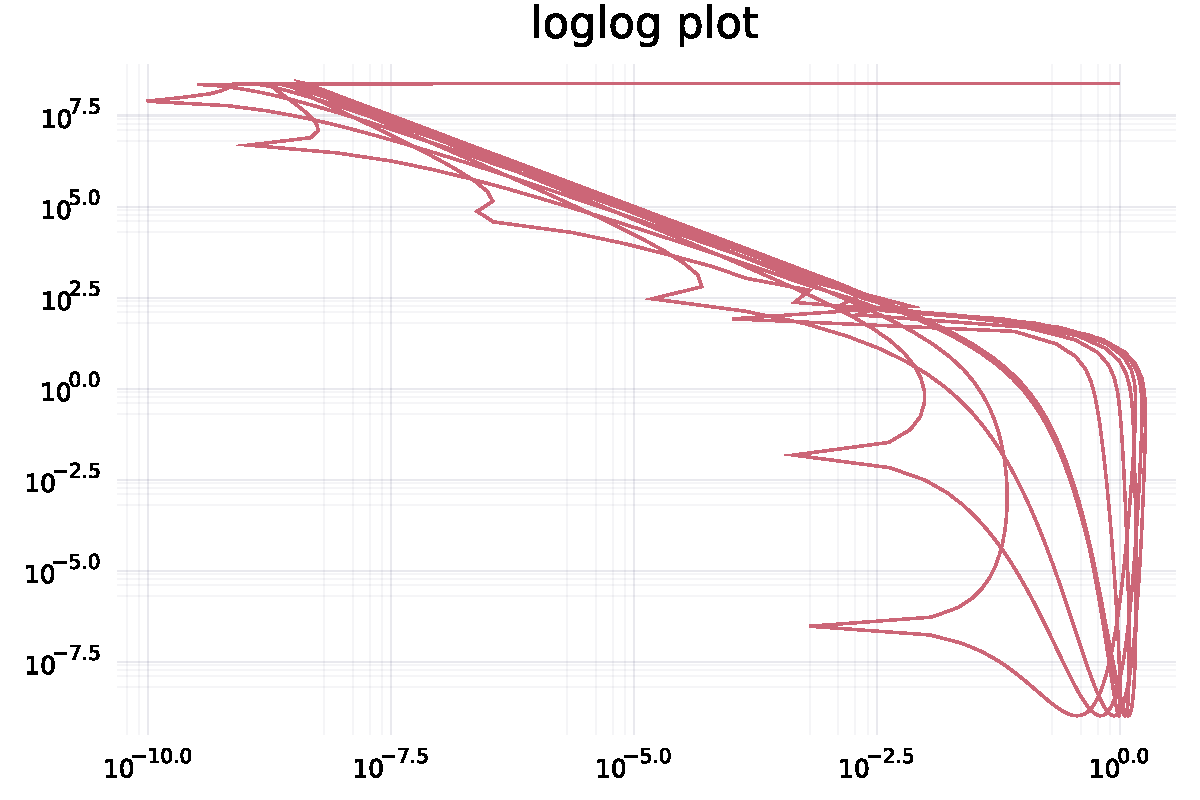
\includegraphics[width=\linewidth]{figures/ass_3_report_8_1.pdf}

\section{Problem 6}

\begin{lstlisting}
(*@\HLJLn{hs}@*) (*@\HLJLoB{=}@*) (*@\HLJLni{1}@*) (*@\HLJLoB{./}@*)(*@\HLJLp{(}@*)(*@\HLJLni{2}@*) (*@\HLJLoB{.{\textasciicircum}}@*)(*@\HLJLp{(}@*)(*@\HLJLni{3}@*)(*@\HLJLoB{:}@*)(*@\HLJLni{8}@*)(*@\HLJLp{))}@*)
(*@\HLJLk{for}@*) (*@\HLJLn{i}@*) (*@\HLJLoB{=}@*) (*@\HLJLni{1}@*) (*@\HLJLoB{:}@*) (*@\HLJLnf{length}@*)(*@\HLJLp{(}@*)(*@\HLJLn{hs}@*)(*@\HLJLp{)}@*)
    (*@\HLJLn{N}@*) (*@\HLJLoB{=}@*) (*@\HLJLnf{Int}@*)(*@\HLJLp{(}@*)(*@\HLJLn{T}@*)(*@\HLJLoB{/}@*)(*@\HLJLn{hs}@*)(*@\HLJLp{[}@*)(*@\HLJLn{i}@*)(*@\HLJLp{])}@*)
    (*@\HLJLn{tList}@*) (*@\HLJLoB{=}@*) (*@\HLJLnf{collect}@*)(*@\HLJLp{(}@*)(*@\HLJLni{0}@*)(*@\HLJLoB{:}@*)(*@\HLJLn{N}@*)(*@\HLJLp{)}@*)(*@\HLJLoB{*}@*)(*@\HLJLp{(}@*)(*@\HLJLn{T}@*)(*@\HLJLoB{/}@*)(*@\HLJLn{N}@*)(*@\HLJLp{)}@*)

    (*@\HLJLcs{{\#}{\#}}@*) (*@\HLJLcs{Backward}@*) (*@\HLJLcs{Euler}@*)
    (*@\HLJLn{u{\_}euler}@*) (*@\HLJLoB{=}@*) (*@\HLJLnf{BackwardEuler{\_}n}@*)(*@\HLJLp{(}@*)(*@\HLJLn{f}@*)(*@\HLJLp{,}@*) (*@\HLJLn{N}@*)(*@\HLJLp{,}@*) (*@\HLJLn{T}@*)(*@\HLJLp{,}@*) (*@\HLJLn{u0}@*)(*@\HLJLp{)}@*)
    (*@\HLJLn{u{\_}eexact}@*) (*@\HLJLoB{=}@*) (*@\HLJLnf{BackwardEuler{\_}n}@*)(*@\HLJLp{(}@*)(*@\HLJLn{f}@*)(*@\HLJLp{,}@*)(*@\HLJLni{2}@*)(*@\HLJLoB{*}@*)(*@\HLJLn{N}@*)(*@\HLJLp{,}@*)(*@\HLJLn{T}@*)(*@\HLJLp{,}@*)(*@\HLJLn{u0}@*)(*@\HLJLp{)}@*)
    (*@\HLJLn{euler{\_}error}@*) (*@\HLJLoB{=}@*) (*@\HLJLn{abs}@*)(*@\HLJLoB{.}@*)(*@\HLJLp{(}@*)(*@\HLJLn{u{\_}euler}@*)(*@\HLJLp{[}@*)(*@\HLJLni{1}@*)(*@\HLJLoB{:}@*)(*@\HLJLn{N}@*)(*@\HLJLp{]}@*) (*@\HLJLoB{-}@*) (*@\HLJLn{u{\_}eexact}@*)(*@\HLJLp{[}@*)(*@\HLJLni{1}@*)(*@\HLJLoB{:}@*)(*@\HLJLni{2}@*)(*@\HLJLoB{:}@*)(*@\HLJLni{2}@*)(*@\HLJLoB{*}@*)(*@\HLJLn{N}@*)(*@\HLJLp{])}@*)(*@\HLJLoB{./}@*)(*@\HLJLp{(}@*)(*@\HLJLni{1}@*)(*@\HLJLoB{-}@*)(*@\HLJLnfB{0.5}@*)(*@\HLJLoB{{\textasciicircum}}@*)(*@\HLJLni{1}@*)(*@\HLJLp{)}@*) (*@\HLJLcs{{\#}}@*) (*@\HLJLcs{first}@*) (*@\HLJLcs{order}@*) (*@\HLJLcs{method}@*)
    (*@\HLJLn{p1}@*) (*@\HLJLoB{=}@*) (*@\HLJLnf{plot}@*)(*@\HLJLp{(}@*)(*@\HLJLn{tList}@*)(*@\HLJLp{[}@*)(*@\HLJLni{2}@*)(*@\HLJLoB{:}@*)(*@\HLJLn{N}@*)(*@\HLJLp{],}@*) (*@\HLJLn{euler{\_}error}@*)(*@\HLJLp{[}@*)(*@\HLJLni{2}@*)(*@\HLJLoB{:}@*)(*@\HLJLn{N}@*)(*@\HLJLp{],}@*) (*@\HLJLn{label}@*) (*@\HLJLoB{=}@*) (*@\HLJLs{"{}Backward}@*) (*@\HLJLs{Euler"{}}@*)(*@\HLJLp{,}@*) (*@\HLJLn{xaxis}@*)(*@\HLJLoB{=:}@*)(*@\HLJLn{log}@*)(*@\HLJLp{,}@*) (*@\HLJLn{yaxis}@*)(*@\HLJLoB{=:}@*)(*@\HLJLn{log}@*)(*@\HLJLp{,}@*) (*@\HLJLn{marker}@*) (*@\HLJLoB{=}@*) (*@\HLJLp{(}@*)(*@\HLJLsc{:square}@*)(*@\HLJLp{,}@*)(*@\HLJLni{5}@*)(*@\HLJLp{))}@*)
    (*@\HLJLnf{xaxis!}@*)(*@\HLJLp{(}@*)(*@\HLJLso{L"{}t"{}}@*)(*@\HLJLp{)}@*)
    (*@\HLJLnf{yaxis!}@*)(*@\HLJLp{(}@*)(*@\HLJLso{L"{}u(t)"{}}@*)(*@\HLJLp{)}@*)
    (*@\HLJLnf{title!}@*)(*@\HLJLp{(}@*)(*@\HLJLnf{latexstring}@*)(*@\HLJLp{(}@*)(*@\HLJLs{"{}Error}@*) (*@\HLJLs{Estimate,h="{}}@*)(*@\HLJLp{,}@*)(*@\HLJLn{hs}@*)(*@\HLJLp{[}@*)(*@\HLJLn{i}@*)(*@\HLJLp{]))}@*)

    (*@\HLJLcs{{\#}{\#}}@*) (*@\HLJLcs{s2-DIRK}@*)
    (*@\HLJLn{u{\_}s2{\_}DIRK}@*) (*@\HLJLoB{=}@*) (*@\HLJLnf{s2{\_}DIRK}@*)(*@\HLJLp{(}@*)(*@\HLJLn{f}@*)(*@\HLJLp{,}@*) (*@\HLJLn{N}@*)(*@\HLJLp{,}@*) (*@\HLJLn{T}@*)(*@\HLJLp{,}@*) (*@\HLJLn{u0}@*)(*@\HLJLp{,}@*) (*@\HLJLn{\ensuremath{\alpha}}@*)(*@\HLJLp{)}@*)
    (*@\HLJLn{u{\_}Dexact}@*) (*@\HLJLoB{=}@*) (*@\HLJLnf{s2{\_}DIRK}@*)(*@\HLJLp{(}@*)(*@\HLJLn{f}@*)(*@\HLJLp{,}@*) (*@\HLJLni{2}@*)(*@\HLJLoB{*}@*)(*@\HLJLn{N}@*)(*@\HLJLp{,}@*) (*@\HLJLn{T}@*)(*@\HLJLp{,}@*) (*@\HLJLn{u0}@*)(*@\HLJLp{,}@*) (*@\HLJLn{\ensuremath{\alpha}}@*)(*@\HLJLp{)}@*)
    (*@\HLJLn{DIRK{\_}error}@*) (*@\HLJLoB{=}@*) (*@\HLJLn{abs}@*)(*@\HLJLoB{.}@*)(*@\HLJLp{(}@*)(*@\HLJLn{u{\_}s2{\_}DIRK}@*)(*@\HLJLp{[}@*)(*@\HLJLni{1}@*)(*@\HLJLoB{:}@*)(*@\HLJLn{N}@*)(*@\HLJLp{]}@*) (*@\HLJLoB{-}@*) (*@\HLJLn{u{\_}Dexact}@*)(*@\HLJLp{[}@*)(*@\HLJLni{1}@*)(*@\HLJLoB{:}@*)(*@\HLJLni{2}@*)(*@\HLJLoB{:}@*)(*@\HLJLni{2}@*)(*@\HLJLoB{*}@*)(*@\HLJLn{N}@*)(*@\HLJLp{])}@*)(*@\HLJLoB{./}@*)(*@\HLJLp{(}@*)(*@\HLJLni{1}@*)(*@\HLJLoB{-}@*)(*@\HLJLnfB{0.5}@*)(*@\HLJLoB{{\textasciicircum}}@*)(*@\HLJLni{2}@*)(*@\HLJLp{)}@*) (*@\HLJLcs{{\#}}@*) (*@\HLJLcs{second}@*) (*@\HLJLcs{order}@*) (*@\HLJLcs{method}@*)
    (*@\HLJLn{p2}@*) (*@\HLJLoB{=}@*) (*@\HLJLnf{plot!}@*)(*@\HLJLp{(}@*)(*@\HLJLn{tList}@*)(*@\HLJLp{[}@*)(*@\HLJLni{2}@*)(*@\HLJLoB{:}@*)(*@\HLJLn{N}@*)(*@\HLJLp{],}@*) (*@\HLJLn{DIRK{\_}error}@*)(*@\HLJLp{[}@*)(*@\HLJLni{2}@*)(*@\HLJLoB{:}@*)(*@\HLJLn{N}@*)(*@\HLJLp{],}@*) (*@\HLJLn{label}@*) (*@\HLJLoB{=}@*) (*@\HLJLs{"{}2s-DIRK}@*) (*@\HLJLs{error"{}}@*)(*@\HLJLp{,}@*) (*@\HLJLn{xaxis}@*)(*@\HLJLoB{=:}@*)(*@\HLJLn{log}@*)(*@\HLJLp{,}@*) (*@\HLJLn{yaxis}@*)(*@\HLJLoB{=:}@*)(*@\HLJLn{log}@*)(*@\HLJLp{,}@*) (*@\HLJLn{marker}@*) (*@\HLJLoB{=}@*) (*@\HLJLp{(}@*)(*@\HLJLsc{:square}@*)(*@\HLJLp{,}@*)(*@\HLJLni{5}@*)(*@\HLJLp{))}@*)
    (*@\HLJLnf{display}@*)(*@\HLJLp{(}@*)(*@\HLJLn{p2}@*)(*@\HLJLp{)}@*)
(*@\HLJLk{end}@*)
\end{lstlisting}

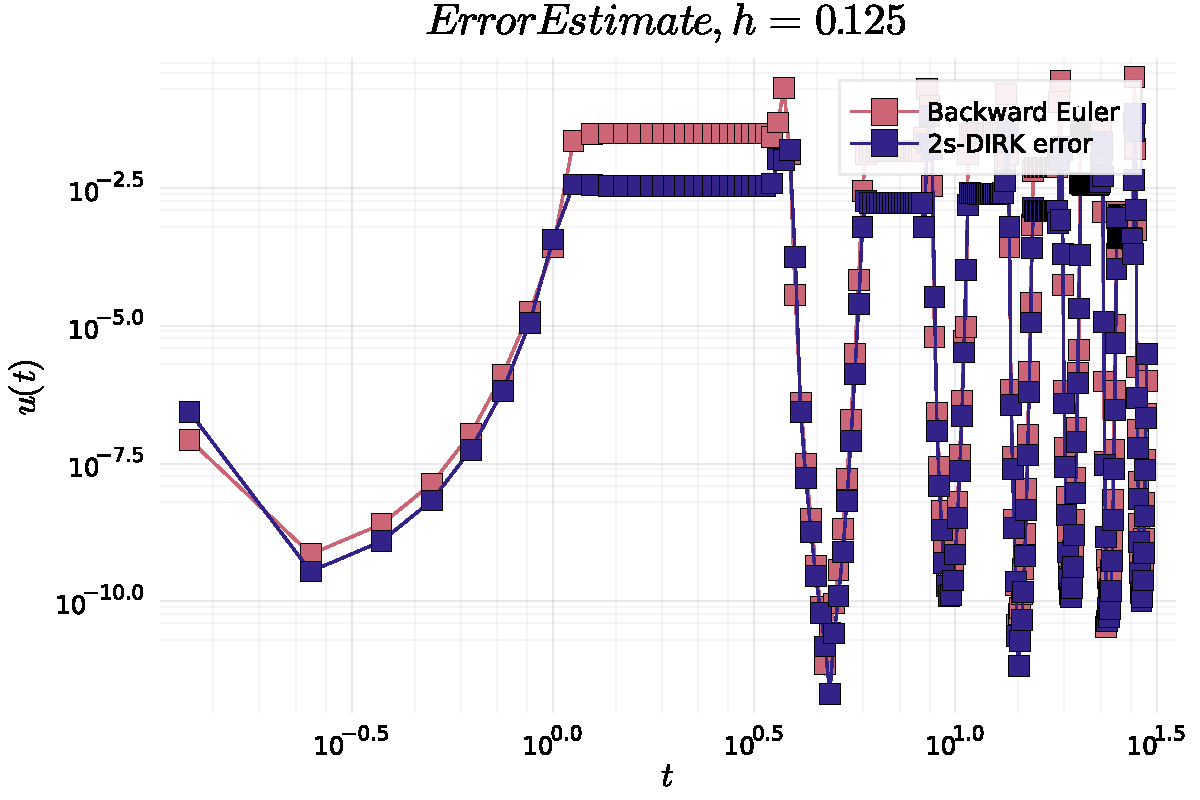
\includegraphics[width=\linewidth]{figures/ass_3_report_9_1.pdf}
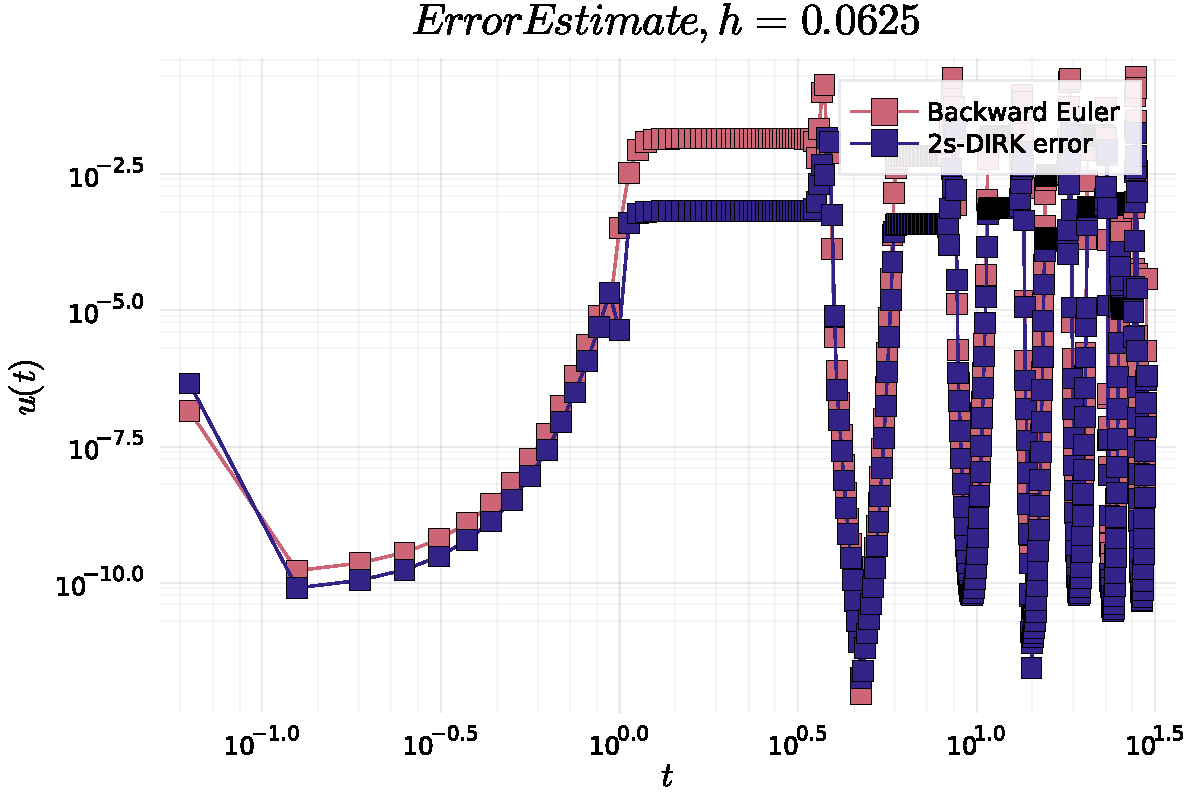
\includegraphics[width=\linewidth]{figures/ass_3_report_9_2.pdf}
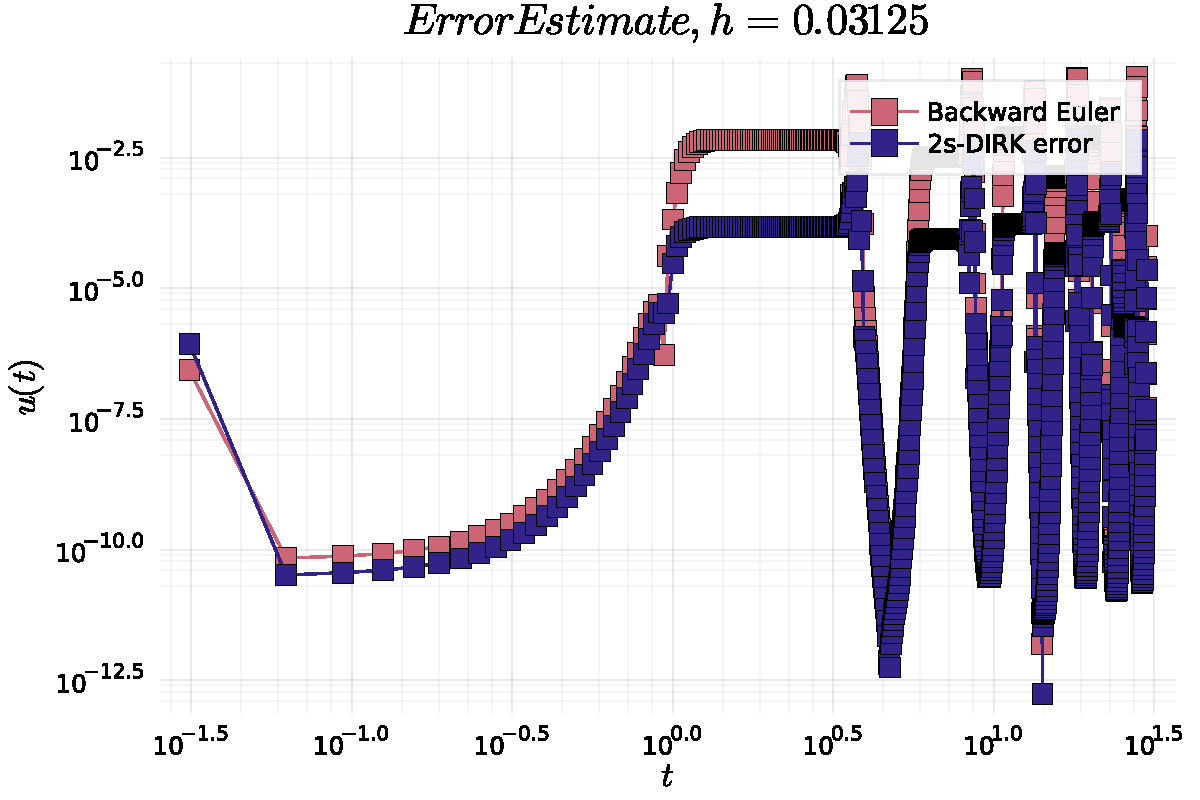
\includegraphics[width=\linewidth]{figures/ass_3_report_9_3.pdf}
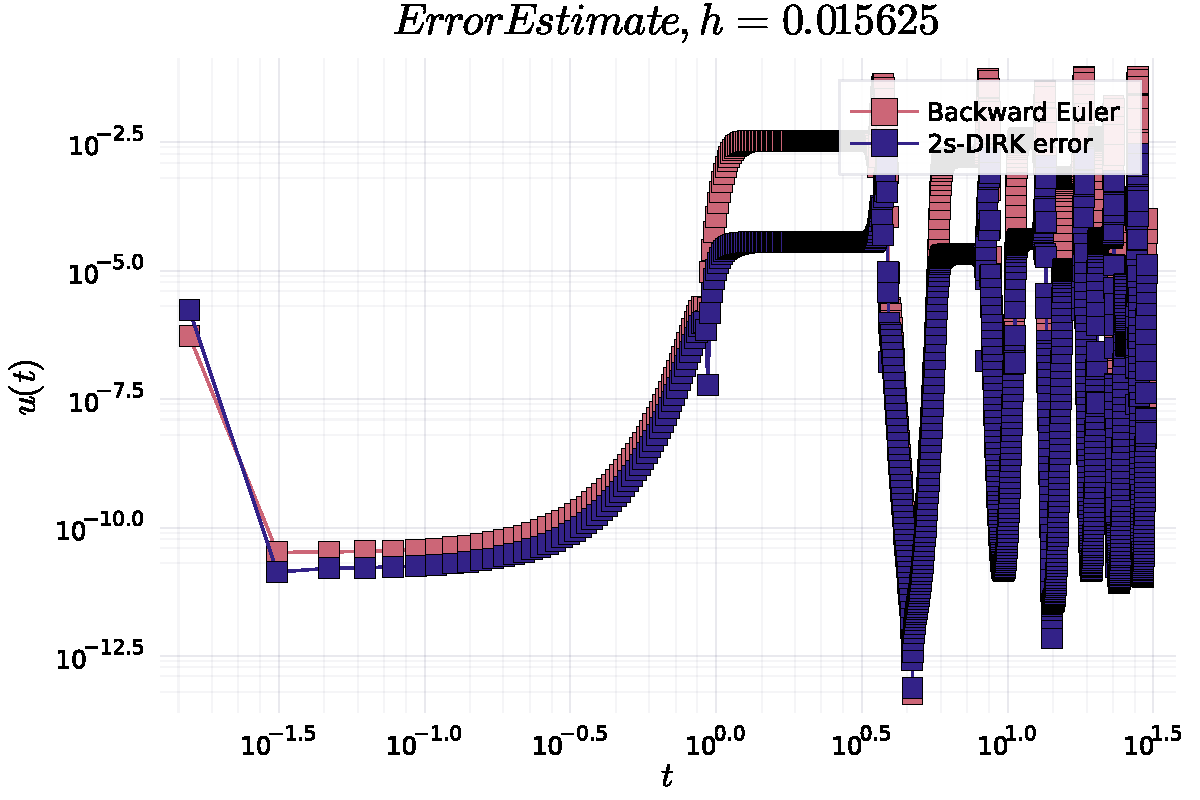
\includegraphics[width=\linewidth]{figures/ass_3_report_9_4.pdf}
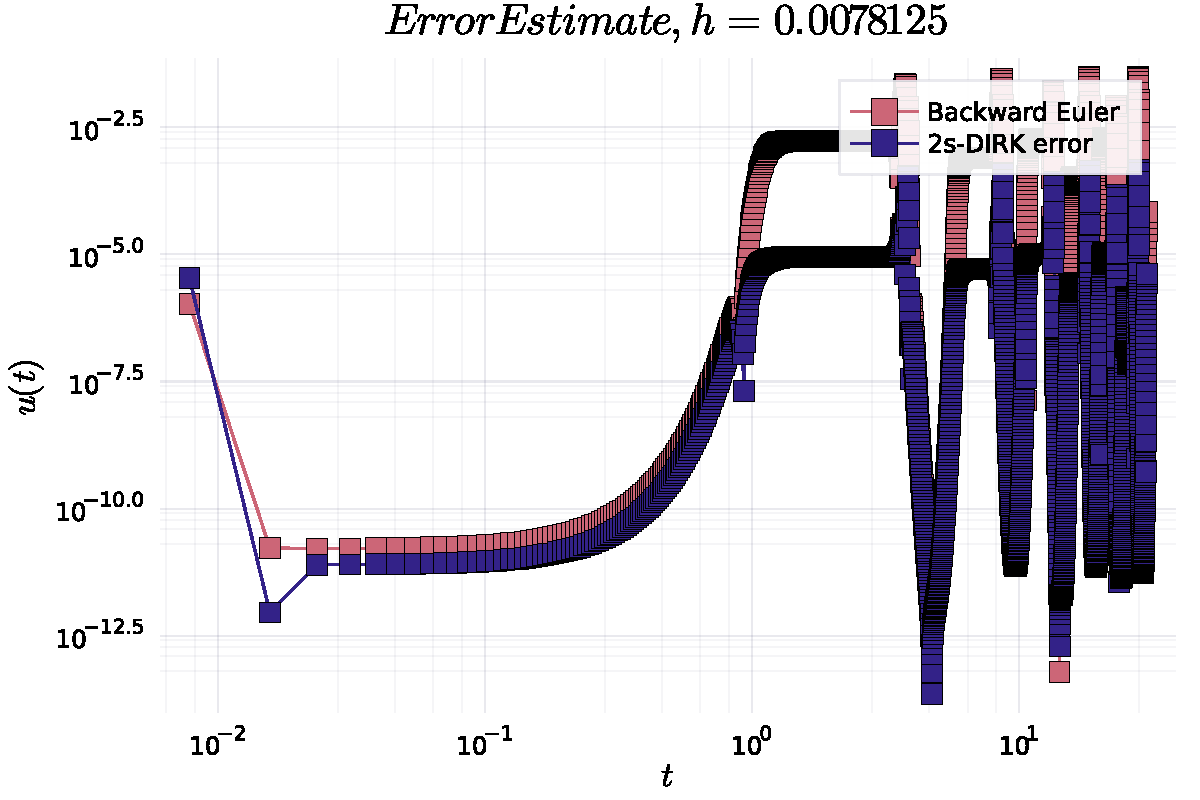
\includegraphics[width=\linewidth]{figures/ass_3_report_9_5.pdf}
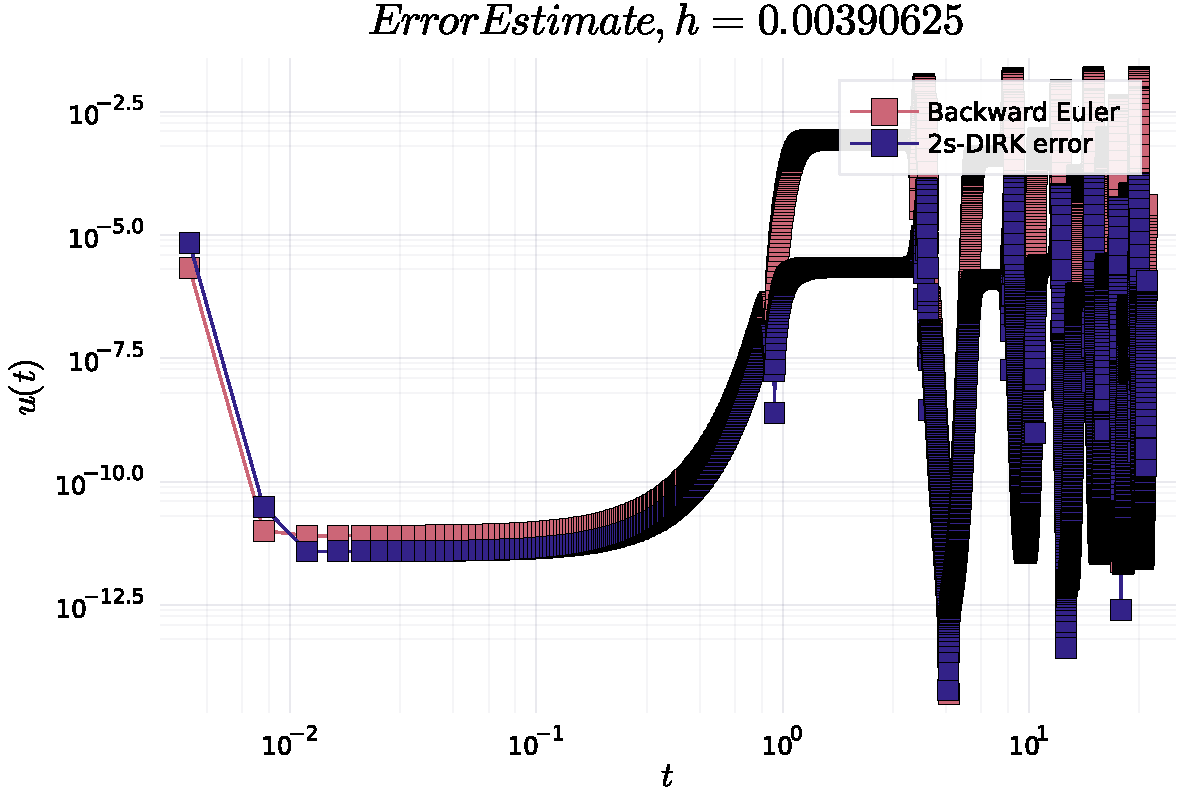
\includegraphics[width=\linewidth]{figures/ass_3_report_9_6.pdf}

\subsubsection{Part 2}

\begin{lstlisting}
(*@\HLJLn{h}@*) (*@\HLJLoB{=}@*) (*@\HLJLnfB{2.0}@*)(*@\HLJLoB{{\textasciicircum}}@*)(*@\HLJLp{(}@*)(*@\HLJLoB{-}@*)(*@\HLJLni{7}@*)(*@\HLJLp{)}@*)
(*@\HLJLn{N}@*) (*@\HLJLoB{=}@*) (*@\HLJLnf{Int}@*)(*@\HLJLp{(}@*)(*@\HLJLn{T}@*)(*@\HLJLoB{/}@*)(*@\HLJLn{h}@*)(*@\HLJLp{)}@*)
(*@\HLJLn{tList}@*) (*@\HLJLoB{=}@*) (*@\HLJLnf{collect}@*)(*@\HLJLp{(}@*)(*@\HLJLni{0}@*)(*@\HLJLoB{:}@*)(*@\HLJLn{N}@*)(*@\HLJLp{)}@*)(*@\HLJLoB{*}@*)(*@\HLJLp{(}@*)(*@\HLJLn{T}@*)(*@\HLJLoB{/}@*)(*@\HLJLn{N}@*)(*@\HLJLp{)}@*)

(*@\HLJLcs{{\#}{\#}}@*) (*@\HLJLcs{Backward}@*) (*@\HLJLcs{Euler}@*)
(*@\HLJLn{u{\_}euler}@*) (*@\HLJLoB{=}@*) (*@\HLJLnf{BackwardEuler{\_}n}@*)(*@\HLJLp{(}@*)(*@\HLJLn{f}@*)(*@\HLJLp{,}@*) (*@\HLJLn{N}@*)(*@\HLJLp{,}@*) (*@\HLJLn{T}@*)(*@\HLJLp{,}@*) (*@\HLJLn{u0}@*)(*@\HLJLp{)}@*)
(*@\HLJLn{u{\_}eexact}@*) (*@\HLJLoB{=}@*) (*@\HLJLnf{BackwardEuler{\_}n}@*)(*@\HLJLp{(}@*)(*@\HLJLn{f}@*)(*@\HLJLp{,}@*)(*@\HLJLni{2}@*)(*@\HLJLoB{*}@*)(*@\HLJLn{N}@*)(*@\HLJLp{,}@*)(*@\HLJLn{T}@*)(*@\HLJLp{,}@*)(*@\HLJLn{u0}@*)(*@\HLJLp{)}@*)
(*@\HLJLn{euler{\_}error}@*) (*@\HLJLoB{=}@*) (*@\HLJLn{abs}@*)(*@\HLJLoB{.}@*)(*@\HLJLp{(}@*)(*@\HLJLn{u{\_}euler}@*)(*@\HLJLp{[}@*)(*@\HLJLni{1}@*)(*@\HLJLoB{:}@*)(*@\HLJLn{N}@*)(*@\HLJLp{]}@*) (*@\HLJLoB{-}@*) (*@\HLJLn{u{\_}eexact}@*)(*@\HLJLp{[}@*)(*@\HLJLni{1}@*)(*@\HLJLoB{:}@*)(*@\HLJLni{2}@*)(*@\HLJLoB{:}@*)(*@\HLJLni{2}@*)(*@\HLJLoB{*}@*)(*@\HLJLn{N}@*)(*@\HLJLp{])}@*)(*@\HLJLoB{./}@*)(*@\HLJLp{(}@*)(*@\HLJLni{1}@*)(*@\HLJLoB{-}@*)(*@\HLJLnfB{0.5}@*)(*@\HLJLoB{{\textasciicircum}}@*)(*@\HLJLni{1}@*)(*@\HLJLp{)}@*) (*@\HLJLcs{{\#}}@*) (*@\HLJLcs{first}@*) (*@\HLJLcs{order}@*) (*@\HLJLcs{method}@*)
(*@\HLJLn{p1}@*) (*@\HLJLoB{=}@*) (*@\HLJLnf{plot}@*)(*@\HLJLp{(}@*)(*@\HLJLn{tList}@*)(*@\HLJLp{[}@*)(*@\HLJLni{2}@*)(*@\HLJLoB{:}@*)(*@\HLJLn{N}@*)(*@\HLJLp{],}@*) (*@\HLJLn{euler{\_}error}@*)(*@\HLJLp{[}@*)(*@\HLJLni{2}@*)(*@\HLJLoB{:}@*)(*@\HLJLn{N}@*)(*@\HLJLp{],}@*) (*@\HLJLn{label}@*) (*@\HLJLoB{=}@*) (*@\HLJLs{"{}Backward}@*) (*@\HLJLs{Euler"{}}@*)(*@\HLJLp{,}@*) (*@\HLJLn{xaxis}@*)(*@\HLJLoB{=:}@*)(*@\HLJLn{log}@*)(*@\HLJLp{,}@*) (*@\HLJLn{yaxis}@*)(*@\HLJLoB{=:}@*)(*@\HLJLn{log}@*)(*@\HLJLp{,}@*) (*@\HLJLn{marker}@*) (*@\HLJLoB{=}@*) (*@\HLJLp{(}@*)(*@\HLJLsc{:square}@*)(*@\HLJLp{,}@*)(*@\HLJLni{5}@*)(*@\HLJLp{))}@*)
(*@\HLJLnf{xaxis!}@*)(*@\HLJLp{(}@*)(*@\HLJLso{L"{}t"{}}@*)(*@\HLJLp{)}@*)
(*@\HLJLnf{yaxis!}@*)(*@\HLJLp{(}@*)(*@\HLJLso{L"{}u(t)"{}}@*)(*@\HLJLp{)}@*)
(*@\HLJLnf{title!}@*)(*@\HLJLp{(}@*)(*@\HLJLnf{latexstring}@*)(*@\HLJLp{(}@*)(*@\HLJLs{"{}Error}@*) (*@\HLJLs{Estimate,h="{}}@*)(*@\HLJLp{,}@*)(*@\HLJLn{h}@*)(*@\HLJLp{))}@*)

(*@\HLJLcs{{\#}{\#}}@*) (*@\HLJLcs{s2-DIRK}@*)
(*@\HLJLn{u{\_}s2{\_}DIRK}@*) (*@\HLJLoB{=}@*) (*@\HLJLnf{s2{\_}DIRK}@*)(*@\HLJLp{(}@*)(*@\HLJLn{f}@*)(*@\HLJLp{,}@*) (*@\HLJLn{N}@*)(*@\HLJLp{,}@*) (*@\HLJLn{T}@*)(*@\HLJLp{,}@*) (*@\HLJLn{u0}@*)(*@\HLJLp{,}@*) (*@\HLJLn{\ensuremath{\alpha}}@*)(*@\HLJLp{)}@*)
(*@\HLJLn{u{\_}Dexact}@*) (*@\HLJLoB{=}@*) (*@\HLJLnf{s2{\_}DIRK}@*)(*@\HLJLp{(}@*)(*@\HLJLn{f}@*)(*@\HLJLp{,}@*) (*@\HLJLni{2}@*)(*@\HLJLoB{*}@*)(*@\HLJLn{N}@*)(*@\HLJLp{,}@*) (*@\HLJLn{T}@*)(*@\HLJLp{,}@*) (*@\HLJLn{u0}@*)(*@\HLJLp{,}@*) (*@\HLJLn{\ensuremath{\alpha}}@*)(*@\HLJLp{)}@*)
(*@\HLJLn{DIRK{\_}error}@*) (*@\HLJLoB{=}@*) (*@\HLJLn{abs}@*)(*@\HLJLoB{.}@*)(*@\HLJLp{(}@*)(*@\HLJLn{u{\_}s2{\_}DIRK}@*)(*@\HLJLp{[}@*)(*@\HLJLni{1}@*)(*@\HLJLoB{:}@*)(*@\HLJLn{N}@*)(*@\HLJLp{]}@*) (*@\HLJLoB{-}@*) (*@\HLJLn{u{\_}Dexact}@*)(*@\HLJLp{[}@*)(*@\HLJLni{1}@*)(*@\HLJLoB{:}@*)(*@\HLJLni{2}@*)(*@\HLJLoB{:}@*)(*@\HLJLni{2}@*)(*@\HLJLoB{*}@*)(*@\HLJLn{N}@*)(*@\HLJLp{])}@*)(*@\HLJLoB{./}@*)(*@\HLJLp{(}@*)(*@\HLJLni{1}@*)(*@\HLJLoB{-}@*)(*@\HLJLnfB{0.5}@*)(*@\HLJLoB{{\textasciicircum}}@*)(*@\HLJLni{2}@*)(*@\HLJLp{)}@*) (*@\HLJLcs{{\#}}@*) (*@\HLJLcs{second}@*) (*@\HLJLcs{order}@*) (*@\HLJLcs{method}@*)
(*@\HLJLn{p2}@*) (*@\HLJLoB{=}@*) (*@\HLJLnf{plot!}@*)(*@\HLJLp{(}@*)(*@\HLJLn{tList}@*)(*@\HLJLp{[}@*)(*@\HLJLni{2}@*)(*@\HLJLoB{:}@*)(*@\HLJLn{N}@*)(*@\HLJLp{],}@*) (*@\HLJLn{DIRK{\_}error}@*)(*@\HLJLp{[}@*)(*@\HLJLni{2}@*)(*@\HLJLoB{:}@*)(*@\HLJLn{N}@*)(*@\HLJLp{],}@*) (*@\HLJLn{label}@*) (*@\HLJLoB{=}@*) (*@\HLJLs{"{}2s-DIRK}@*) (*@\HLJLs{error"{}}@*)(*@\HLJLp{,}@*) (*@\HLJLn{xaxis}@*)(*@\HLJLoB{=:}@*)(*@\HLJLn{log}@*)(*@\HLJLp{,}@*) (*@\HLJLn{yaxis}@*)(*@\HLJLoB{=:}@*)(*@\HLJLn{log}@*)(*@\HLJLp{,}@*) (*@\HLJLn{marker}@*) (*@\HLJLoB{=}@*) (*@\HLJLp{(}@*)(*@\HLJLsc{:square}@*)(*@\HLJLp{,}@*)(*@\HLJLni{5}@*)(*@\HLJLp{))}@*)
(*@\HLJLnf{display}@*)(*@\HLJLp{(}@*)(*@\HLJLn{p2}@*)(*@\HLJLp{)}@*)
\end{lstlisting}

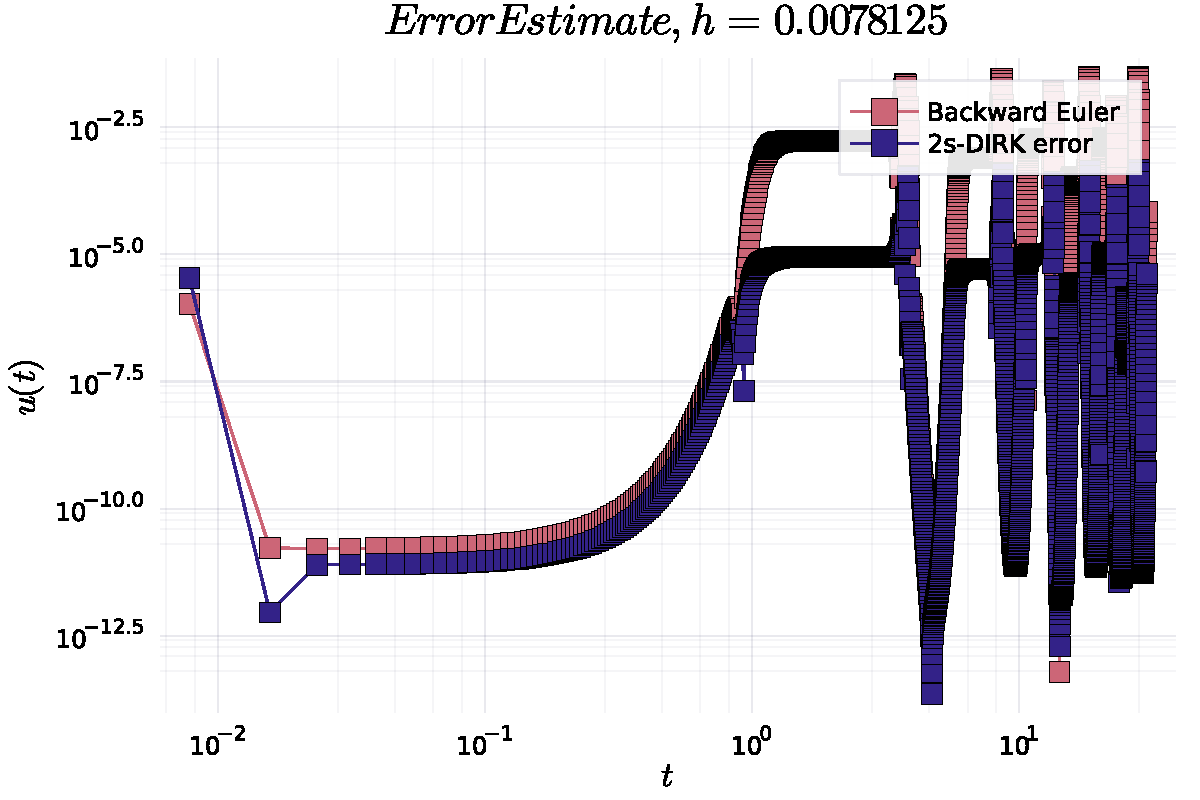
\includegraphics[width=\linewidth]{figures/ass_3_report_10_1.pdf}


\end{document}
